% !TeX program = xelatex
% !BIB program = biber
\makeatletter
\def\input@path{{vendor/tex-packages/footmisc/tex/latex/footmisc/}{vendor/tex-packages/appendix/tex/latex/appendix/}{vendor/tex-packages/multirow/tex/latex/multirow/}{vendor/tex-packages/placeins/tex/latex/placeins/}{vendor/tex-packages/abstract/tex/latex/abstract/}}
\makeatother
\documentclass[lang=cn,11pt,a4paper,math=cm,bibstyle=gb7714-2015,citestyle=gb7714-2015]{elegantpaper}
\usepackage{tabularx,array,flafter}
\usepackage[section]{placeins}
\ExecuteBibliographyOptions{sorting=none,doi=true,url=false,isbn=false,maxbibnames=3,minbibnames=3}
\addbibresource{references.bib}
\hypersetup{colorlinks=true,linkcolor=black,citecolor=black,urlcolor=black,
 pdftitle={基于人工特征与时序特征融合的跨受试者人体活动识别研究}}
\graphicspath{{figures/}}
\setlength{\emergencystretch}{2em}
\clubpenalty=10000
\widowpenalty=10000
\displaywidowpenalty=10000
\raggedbottom
\renewcommand{\topfraction}{0.9}
\renewcommand{\bottomfraction}{0.8}
\renewcommand{\textfraction}{0.1}
\renewcommand{\floatpagefraction}{0.7}
\setlength{\textfloatsep}{14pt plus 3pt minus 3pt}
\setlength{\floatsep}{12pt plus 2pt minus 2pt}
\captionsetup{font=small}
\newcommand{\tabnote}[1]{\par\vspace{3pt}{\footnotesize #1\par}}
\newcolumntype{Y}{>{\raggedright\arraybackslash}X}
\title{基于人工特征与时序特征融合的\\跨受试者人体活动识别研究}
% 请自行填写真实信息；空白值不会在论文中伪造署名。
\author{}
\institute{} % 可填写班级与学号
\date{}

\begin{document}
\maketitle
\begin{center}\small\bfseries Cross-Subject Human Activity Recognition via Fusion of Handcrafted and Temporal Features\end{center}
\begin{abstract}
针对智能手机人体活动识别中不同受试者之间的分布差异，本文基于 UCI HAR 数据集开展监督分类研究。将数据集提供的 561 维人工特征与九通道惯性时间序列对齐，构建多层感知机与一维卷积神经网络的双分支拼接融合模型，并设置逻辑回归、支持向量机、随机森林及单分支神经网络作为对照。采用按受试者划分的五折交叉验证，神经网络通过内层受试者验证选择训练轮数；模型与配置冻结后，在官方独立测试集上评价。逻辑回归取得最高的交叉验证宏平均 F1（0.9339），融合模型为 0.9318。独立测试中，逻辑回归与融合模型的宏平均 F1 分别为 0.9500 和 0.9564，融合模型净减少 17 个错误，但坐与站立类别的 F1 下降。结果表明，两种表示的融合在本次测试中改善了总体识别性能，仍存在类别间收益不均与跨受试者波动。本文的贡献在于统一分组协议下的实证比较、稳定性复验及误差分析，不将常见拼接结构视为新架构。
\keywords{人体活动识别；监督学习；跨受试者验证；特征融合；一维卷积神经网络}
\end{abstract}
\noindent\textbf{Abstract:} This study evaluates supervised human activity recognition on UCI HAR under subject-disjoint splits. A two-branch network combines a multilayer perceptron for 561 handcrafted features with a one-dimensional convolutional encoder for nine-channel inertial sequences. Logistic regression, support vector machines, random forests, and single-branch networks serve as comparison models. Five-fold subject-grouped cross-validation is used for development, with inner subject validation selecting neural training epochs. After configurations are frozen, logistic regression and the fusion model achieve test macro-F1 scores of 0.9500 and 0.9564, respectively. Fusion produces 17 fewer errors overall, while reducing F1 for sitting and standing. Logistic regression retains the highest cross-validation mean. These findings support a limited, dataset-specific benefit of representation fusion rather than universal superiority.\par
\vspace{4pt}\noindent\textbf{Key words:} human activity recognition; supervised learning; cross-subject validation; feature fusion; one-dimensional convolution\par
\clearpage
\section{引言}
人体活动识别旨在根据传感器观测判断人的运动状态，是移动健康与人机交互中的基础任务。智能手机惯性传感器能够连续记录加速度和角速度，但同一活动在不同人的动作幅度、节奏与姿态下可能产生不同信号。因此，评价模型时需要关注其对未参与训练的受试者的识别能力，不能仅依赖同一批受试者内部的随机窗口划分。

UCI HAR 为此提供了同时包含人工特征和惯性信号窗口的公开数据资源\cite{uci,anguita2013}。人工特征将时域与频域统计信息压缩为固定维数表示，适合传统分类器；时序网络则能够直接从窗口序列中学习局部变化模式。支持向量机与随机森林分别代表核方法和树集成方法\cite{cortes1995,breiman2001}。可穿戴活动识别中的卷积与循环网络研究说明了从信号学习表示的可行性\cite{ordonez2016}，但不同数据集、输入通道及划分协议下的分数不能直接作为统一排名依据。

本文考察人工特征表示与学习得到的时序表示是否具有互补性。以逻辑回归为强基准，构建常见的 MLP--CNN 双分支拼接网络，并在同一组外层受试者划分上比较六类模型。研究包括人工特征降维对照、融合模型的随机种子复验，以及冻结模型后的官方独立测试。重点回答三个问题：融合是否改善验证和测试表现；降维是否带来性能与计算开销的折中；总体指标的变化是否同时惠及所有类别和受试者。本文采用的拼接机制属于通用表示融合方法，研究价值主要体现在可追溯的实验流程和对收益边界的分析。

\section{数据描述与任务定义}
数据集由 30 名受试者佩戴腰部智能手机完成六类活动，采样频率为 50 Hz，采用长度为 2.56 s、含 128 个采样点且相邻窗口重叠 50\% 的窗口构造样本\cite{uci,anguita2013}。本文沿用官方按受试者划分的训练集与测试集：训练集含 21 人、7352 个窗口，测试集含另外 9 人、2947 个窗口。检查结果表明，两集合的受试者交集为空，训练特征均为有限数值；各类别数量见表\ref{tab:data}。
\begin{table}[htbp]\centering\small
\caption{官方训练集与测试集的类别分布}\label{tab:data}
\begin{tabular}{lrrr}\toprule
类别 & 训练窗口数 & 测试窗口数 & 总数\\\midrule
步行 & 1226 & 496 & 1722\\
上楼 & 1073 & 471 & 1544\\
下楼 & 986 & 420 & 1406\\
坐 & 1286 & 491 & 1777\\
站立 & 1374 & 532 & 1906\\
躺卧 & 1407 & 537 & 1944\\
合计 & 7352 & 2947 & 10299\\
\bottomrule\end{tabular}
\end{table}


记第 $i$ 个窗口为 $(\boldsymbol{x}_i,\boldsymbol{S}_i,y_i,g_i)$，其中 $\boldsymbol{x}_i\in\mathbb{R}^{561}$ 为人工特征，$\boldsymbol{S}_i\in\mathbb{R}^{9\times128}$ 为时序信号，$y_i\in\{1,\ldots,6\}$ 为活动标签，$g_i$ 为受试者编号。九个通道依次为三轴身体加速度、三轴角速度和三轴总加速度。两种输入按同一窗口的行号对齐，分类目标是学习从输入到六类活动的映射。

人工特征及预处理后的信号窗口均由数据集发布者提供，本文没有重新执行连续信号去噪、切窗或人工特征提取。神经网络实现将标签减一编码为 $0$ 至 $5$，报告时恢复原活动名称。两条分支使用同一窗口的不同表示，因而称为表示或特征融合；它们不构成独立采集的两种传感器模态。

\section{模型描述}
\subsection{标准化与传统分类器}
为消除特征尺度差异，对人工特征第 $j$ 维执行
\begin{equation}
 z_{ij}=\frac{x_{ij}-\mu_j}{\widetilde\sigma_j},\qquad
 \widetilde\sigma_j=\begin{cases}\sigma_j,&\sigma_j>0,\\1,&\sigma_j=0.\end{cases}
\end{equation}
均值和标准差仅由当前训练部分估计。逻辑回归使用多类线性判别与交叉熵拟合，$C$ 控制正则化强度的倒数。SVM 采用径向基核 $K(\boldsymbol{z},\boldsymbol{z}')=\exp(-\gamma\|\boldsymbol{z}-\boldsymbol{z}'\|_2^2)$，调整 $C$ 与 $\gamma$\cite{cortes1995}。随机森林集成 200 棵树，调整树深度及叶节点最小样本数，不额外执行标准化\cite{breiman2001}。

另以固定 $C=0.1$ 的逻辑回归考察主成分分析（PCA）。在每折训练部分内拟合标准化器与 PCA，再变换验证数据；分别保留 90\%、95\% 和 99\% 的累计解释方差。PCA 以方差保留为目标，并不直接最大化类别可分性\cite{jolliffe2016}，因此降维后的分类效果需要通过实验判断。

\subsection{单分支神经网络}
MLP 以标准化人工特征为输入，依次经过 $561\to128\to64\to6$ 的全连接层；两个隐藏层后均使用 ReLU 和丢弃率为 0.3 的 Dropout\cite{dropout2014}。该网络包含 80582 个可训练参数，作为人工特征的非线性分类对照。

1D CNN 沿时间轴卷积，三层通道数依次为 $9\to32\to64\to128$，卷积核宽度为 $7,5,3$，步长为 1，并采用保持时间长度的填充。各卷积层后接批归一化（BN）\cite{ioffe2015}与 ReLU，前两层再接宽度为 2 的最大池化，使时间长度依次由 128 变为 64、32。最后使用全局平均池化、Dropout（0.3）与 $128\to6$ 线性分类层。可训练参数共 38278 个。该网络使用提供的惯性信号窗口，而不使用 561 维人工特征。

\subsection{双分支特征融合}
融合模型保留上述 MLP 的 64 维隐藏表示与 CNN 的 128 维池化表示，去除各自最终分类层，将两表示拼接后送入六类线性分类器。结构见图\ref{fig:architecture}，可训练参数共 118854 个。对于信号通道 $c$，先在当前训练窗口及时间轴上计算 $\mu_c^{S},\sigma_c^{S}$，并执行
\begin{equation}
 \widetilde S_{ict}=\frac{S_{ict}-\mu_c^{S}}{\max(\sigma_c^{S},10^{-6})}.
\end{equation}
融合及预测过程写为
\begin{align}
 \boldsymbol h_i^{f}&=f_{\theta}(\boldsymbol z_i)\in\mathbb R^{64}, &
 \boldsymbol h_i^{s}&=g_{\phi}(\widetilde{\boldsymbol S}_i)\in\mathbb R^{128},\\
 \boldsymbol a_i&=W_o[\boldsymbol h_i^{f};\boldsymbol h_i^{s}]+\boldsymbol b_o, &
 p_{ik}&=\frac{\exp(a_{ik})}{\sum_{r=1}^{6}\exp(a_{ir})}.
\end{align}
其中分号表示拼接，训练损失为
\begin{equation}
 \mathcal L=-\frac1N\sum_{i=1}^{N}\log p_{i,y_i}.
\end{equation}
实现中将未经过 softmax 的 logits 输入交叉熵函数，预测取最大分数类别。两分支从头联合训练，未采用预训练、注意力或循环模块。优化器使用 AdamW 的解耦权重衰减\cite{adamw2019}。
\begin{figure}[htbp]\centering
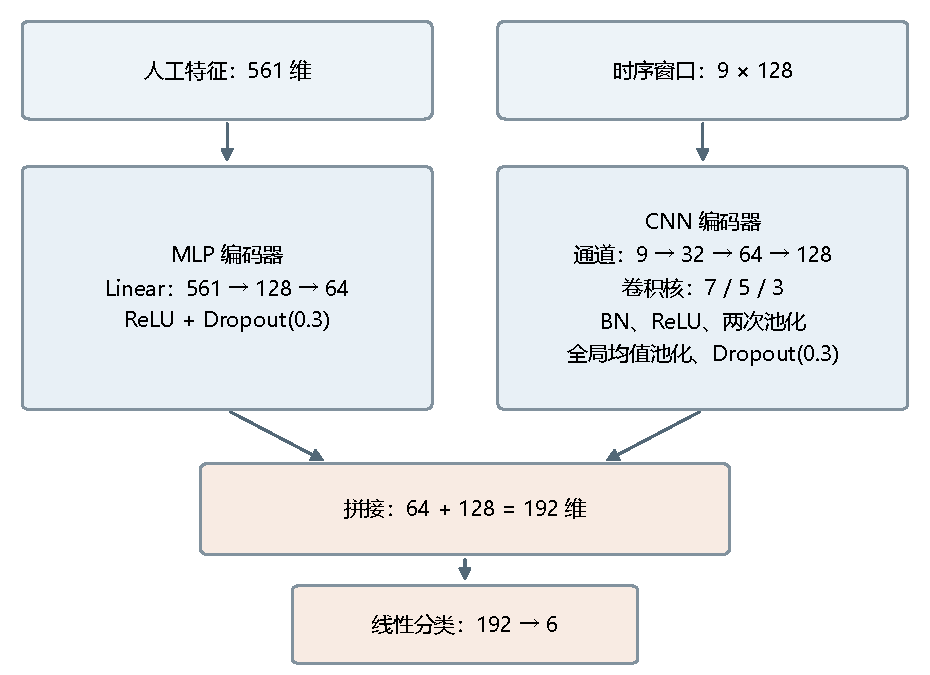
\includegraphics[width=\linewidth]{architecture.pdf}
\caption{双分支融合网络。人工特征与时间序列来自同一窗口；拼接表示维数为 192。}\label{fig:architecture}
\end{figure}

\section{实验设置与评价协议}
\subsection{受试者分组与模型选择}
仅在官方训练集内使用五折 GroupKFold，将同一受试者的全部窗口放入同一折。五个外层验证组依次包含受试者 $\{14,15,19,25\}$、$\{6,16,21,22\}$、$\{3,11,17,26\}$、$\{1,7,23,30\}$ 和 $\{5,8,27,28,29\}$，对应验证窗口数为 1420、1420、1417、1410、1685。六类模型使用相同外层划分，避免重叠窗口跨训练与验证集合共享同一人的信息。

传统模型按表\ref{tab:grid}的网格搜索，以五折宏平均 F1 选择参数，逻辑回归最大迭代次数为 3000，随机森林随机种子为 42。标准化器放在分类流水线内，在每折训练部分拟合。这里的五折分数同时用于选择传统模型超参数与报告开发结果，存在选择乐观性，并非完全嵌套交叉验证的无偏泛化估计。
\begin{table}[tbp]\centering\small
\caption{传统分类器搜索空间与选定参数}\label{tab:grid}
\begin{tabularx}{\linewidth}{lYY}\toprule
模型 & 搜索空间 & 选定参数\\\midrule
逻辑回归 & $C\in\{0.001,0.01,0.1,1,10\}$ & $C=0.1$\\
RBF SVM & $C\in\{1,10,100\}$；$\gamma\in\{\texttt{scale},0.001,0.01\}$ & $C=10,\ \gamma=0.001$\\
随机森林 & 深度 $\in\{\text{不限},20\}$；叶节点最小样本数 $\in\{1,3\}$ & 深度 20；最小样本数 3\\\bottomrule
\end{tabularx}
\end{table}

神经网络结构保持固定，每个外层训练集再用 GroupShuffleSplit 划出约 20\% 的受试者作为内层验证组，划分种子固定为 42。此比例指受试者比例，不要求窗口数恰为 20\%。首先仅用内层训练部分拟合预处理参数并训练，按内层宏平均 F1 选择轮数。上限为 100 轮，连续 10 轮无严格提升即停止。随后重新初始化网络，在全部外层训练数据上重新拟合标准化参数，并按选定轮数重训，最后仅评价一次外层验证集。外层验证分数不参与该折的早停。

三类神经网络均使用批量大小 128、学习率 $10^{-3}$、权重衰减 $10^{-4}$ 和交叉熵损失。基础种子为 42 时，第 $k$ 折训练种子为 $42+k-1$。融合模型另外使用基础种子 2024、2025 复验，保持数据划分、结构和优化设置一致，仅改变初始化及训练随机性。推断时使用评价模式，关闭 Dropout，并使用 BN 的运行统计量。

\subsection{最终训练与独立测试}
根据训练集开发结果，在查看官方测试标签对应的预测成绩前，将逻辑回归 $C=0.1$、不使用 PCA 固定为主基准，融合模型固定为比较模型。融合最终轮数取三个基础种子共 15 个内层所选轮数的中位数 9，最终训练种子固定为 42。两模型用完整的 7352 个训练窗口重新训练并保存模型、预处理参数及配置，随后加载这些文件对 2947 个官方测试窗口进行预测。测试时不重新拟合标准化器或更新模型权重。本次仅对这两个冻结模型实施独立测试。

\subsection{指标与实现环境}
以准确率和宏平均 F1 为主要指标，六个类别等权。令 $TP_c,FP_c,FN_c$ 分别表示类别 $c$ 的真阳性、假阳性和假阴性数量，则
\begin{equation}
 \mathrm{Accuracy}=\frac{\sum_i\mathbf1(\widehat y_i=y_i)}{N},\quad
 F_{1,c}=\frac{2TP_c}{2TP_c+FP_c+FN_c},\quad
 F_{1,\mathrm{macro}}=\frac16\sum_{c=1}^{6}F_{1,c}.
\end{equation}
分母为零时按实现约定将相应 F1 记为零。五折分数按折等权求均值，折间标准差使用总体形式（ddof=0），不能视为独立测试指标或置信区间。三次复验则对三个五折均值另算样本标准差（ddof=1），与折间波动分别报告。

实验在 Windows 的 Python 3.14.3 环境执行，NumPy、scikit-learn 与 PyTorch 版本分别为 2.5.4、1.9.1 和 2.14.1+cpu，采用 CPU 计算。神经网络设置四个计算线程，DataLoader 工作进程数为零。传统分类器与深度学习分别基于 scikit-learn\cite{sklearn2011}和 PyTorch\cite{pytorch2019}。各阶段结果以 CSV/JSON、逐样本预测和模型文件留档；绘图与论文表格从这些结果文件生成，不重新训练或预测。文中耗时仅描述本机单次运行，不作为严格控制条件下的计算效率排名。

\section{实验结果与分析}
\subsection{五折模型比较}
表\ref{tab:cv}与图\ref{fig:cv}给出六类模型的训练集开发结果。逻辑回归的宏平均 F1 为 0.9339，融合模型为 0.9318，二者均值差为 0.0021，远小于各自约 0.04 的折间标准差。单次基础种子 42 下，融合比 MLP 和 CNN 的均值分别高约 0.0032 和 0.0077；这些差异尚不能证明显著提升。
\begin{table}[htbp]\centering\small
\caption{六类模型的五折分组开发结果}\label{tab:cv}
\begin{tabular}{lrrr}\toprule
模型 & 训练 F1 均值 & 验证 F1 均值 & 折间标准差\\\midrule
逻辑回归 & 0.9934 & 0.9339 & 0.0427\\
SVM & 0.9962 & 0.9292 & 0.0389\\
随机森林 & 0.9999 & 0.9165 & 0.0453\\
MLP & 0.9939 & 0.9286 & 0.0427\\
1D CNN & 0.9656 & 0.9241 & 0.0438\\
融合模型 & 0.9807 & 0.9318 & 0.0438\\
\bottomrule\end{tabular}
\tabnote{F1 均为宏平均；神经网络基础种子为 42。传统模型在同一组折上搜索参数，分数存在选择乐观性。}
\end{table}

\begin{figure}[htbp]\centering
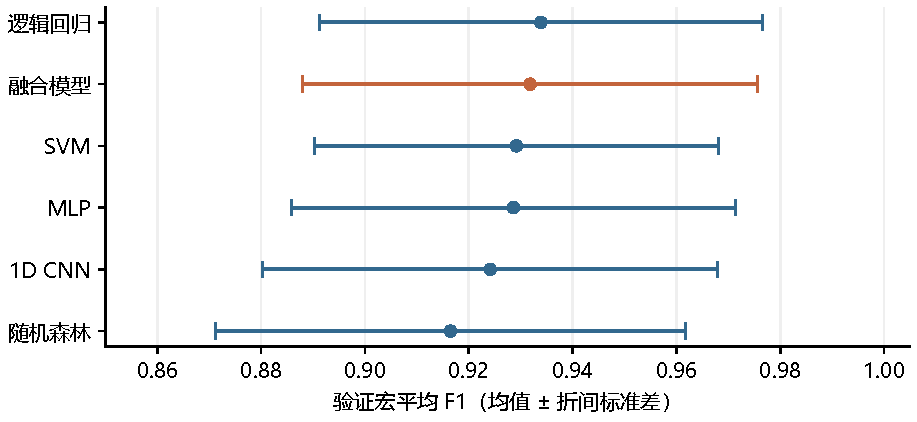
\includegraphics[width=.88\linewidth]{cv_comparison.pdf}
\caption{训练集五折分组交叉验证的宏平均 F1。误差线为折间标准差（ddof=0），不是置信区间；神经网络使用基础种子 42。}\label{fig:cv}
\end{figure}

逻辑回归、MLP 与融合模型的训练 F1 均明显高于验证 F1，反映了拟合训练窗口与识别新受试者之间的差距；随机森林训练 F1 接近 1，验证均值却最低。模型容量增加没有保证跨受试者性能同步提升。融合网络在第 1、2 折的验证 F1 分别约为 0.8910、0.9013，在第 3、4 折则约为 0.9900、0.9804，说明不同验证受试者组合与显著不同的难度相伴随，但现有实验不足以分离体态、动作习惯或采集条件各自的影响。

\subsection{正则化与 PCA 对照}
逻辑回归在 $C=0.001$ 时的验证宏平均 F1 为 0.9130，$C=0.1$ 时达到 0.9339，增至 $C=10$ 后降至 0.9280，而训练 F1 上升至约 0.9998。这说明在本次搜索范围内，适中的正则化取得了较好折中。RBF SVM 在 $\gamma=0.01$ 时训练 F1 接近 1，验证 F1 约为 0.84，也呈现明显的训练与验证差距。
\begin{table}[htbp]\centering\small
\caption{固定逻辑回归 $C=0.1$ 的 PCA 对照}\label{tab:pca}
\begin{tabular}{lrrrr}\toprule
设置 & 各折维数范围 & 验证 F1 & 折间标准差 & 耗时/s\\\midrule
不使用 PCA & 561 & 0.9339 & 0.0427 & 218.9\\
PCA 90\% & 62 & 0.9036 & 0.0537 & 83.9\\
PCA 95\% & 100--101 & 0.9205 & 0.0455 & 56.4\\
PCA 99\% & 177--178 & 0.9280 & 0.0443 & 262.6\\
\bottomrule\end{tabular}
\tabnote{保留比例指累计解释方差；各设置未重新搜索分类器参数，耗时为本机单次五折运行记录。}
\end{table}


表\ref{tab:pca}中，保留 95\% 方差将维数减少至约 100，但验证 F1 降至 0.9205；保留 99\% 方差时为 0.9280，仍低于不降维结果。可能的解释是，较低方差的方向中仍含有分类所需信息。不过，本实验对各 PCA 设置固定 $C=0.1$，未分别重新调参，因此只能评价当前组合，不能证明 PCA 对该任务普遍无效。95\% 设置的单次运行耗时较短，但 99\% 设置反而更慢，提示求解迭代与系统状态也会影响耗时。

\subsection{融合模型的随机性复验}
\begin{table}[htbp]\centering\small
\caption{融合模型三个基础种子的分组验证结果}\label{tab:seeds}
\begin{tabular}{lrrl}\toprule
基础种子 & 五折平均 F1 & 折间标准差 & 各折选定轮数\\\midrule
42 & 0.9318 & 0.0438 & 11, 9, 16, 3, 1\\
2024 & 0.9330 & 0.0433 & 9, 11, 29, 10, 6\\
2025 & 0.9295 & 0.0374 & 6, 11, 17, 3, 1\\
\bottomrule\end{tabular}
\tabnote{三次五折均值平均为 0.9314，均值间样本标准差（ddof=1）为 0.0018；外层与内层受试者划分均固定。}
\end{table}

三个基础种子对应的五折均值平均为 0.9314，均值之间的样本标准差为 0.0018，低于各次运行约 0.0374--0.0438 的折间标准差。这表明在固定受试者划分下，所观察的初始化及批次随机性波动小于受试者组合间的分数波动；它不等价于对任意受试者划分都稳定。部分内层选择轮数仅为 1 或 3，也提示早停对特定内层受试者组合较敏感。由于 MLP 与 CNN 未做相同次数的多种子复验，这里不将融合相对于单分支的差值解释为稳健优势。

\subsection{官方独立测试与类别误差}
\begin{table}[htbp]\centering\small
\caption{冻结模型的官方独立测试结果}\label{tab:test}
\begin{tabular}{lrrr}\toprule
模型 & 准确率 & 宏平均 F1 & 错误窗口数\\\midrule
逻辑回归 & 0.9498 & 0.9500 & 148\\
融合模型 & 0.9555 & 0.9564 & 131\\
\bottomrule\end{tabular}
\tabnote{共 2947 个窗口、9 名受试者。两模型配置均在独立测试前固定。}
\end{table}

冻结后的测试结果见表\ref{tab:test}。融合的准确率比逻辑回归高 0.58 个百分点，宏平均 F1 高 0.64 个百分点，错误数从 148 减至 131。交叉验证均值与独立测试的相对排序不同，说明两种评价所涉及的受试者组合可能影响结论；不能使用测试结果回头改变此前的模型选择规则。

逐样本配对比较显示，两模型共同识别正确 2754 个窗口，共同出错 86 个；融合修正了逻辑回归的 62 个错误，同时新增了 45 个逻辑回归原本识别正确的错误，净改善为 17 个。按测试受试者统计，融合的准确率在 6 人上提高、2 人上降低、1 人上相同；例如受试者 10 从 82.65\% 降至 77.55\%。因此，总体均值提升不能表述为每名受试者均受益。两个模型的混淆矩阵见图\ref{fig:cm-lr}、图\ref{fig:cm-fusion}，各类别 F1 见图\ref{fig:class}。
\begin{figure}[htbp]\centering
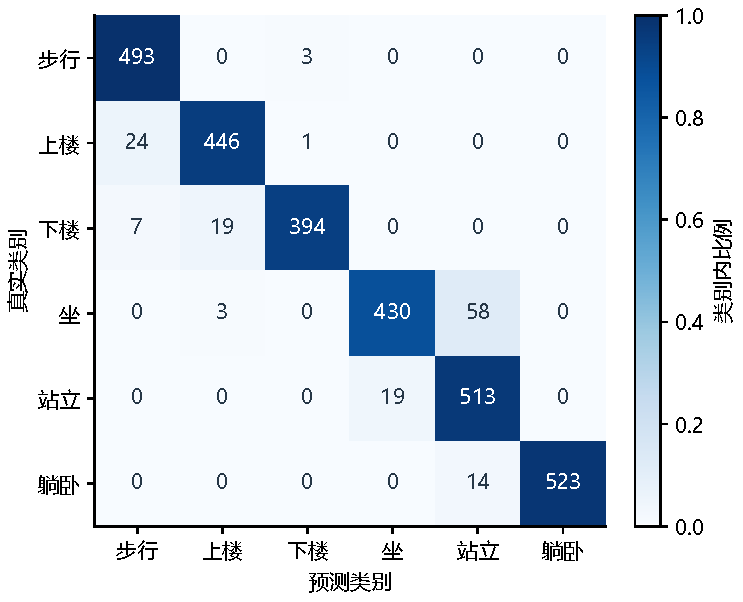
\includegraphics[width=.78\linewidth]{cm_logistic.pdf}
\caption{逻辑回归的独立测试混淆矩阵。行表示真实类别，列表示预测类别；数字为样本数，颜色按真实类别逐行归一化。}\label{fig:cm-lr}
\end{figure}
\begin{figure}[htbp]\centering
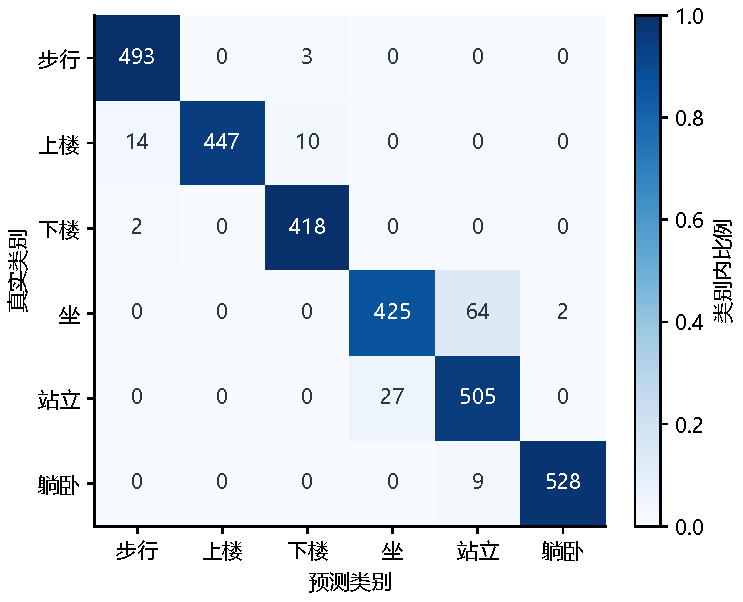
\includegraphics[width=.78\linewidth]{cm_fusion.pdf}
\caption{融合模型的独立测试混淆矩阵。与图\ref{fig:cm-lr}采用相同归一化方式和颜色范围。}\label{fig:cm-fusion}
\end{figure}
\begin{figure}[htbp]\centering
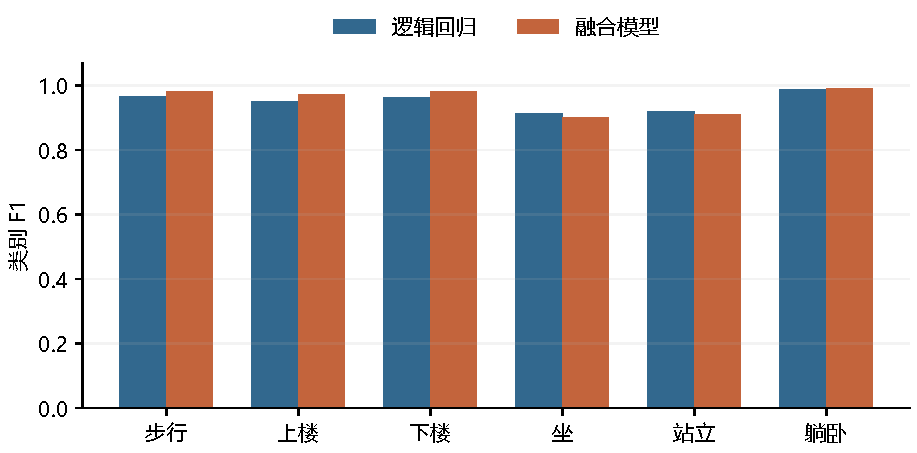
\includegraphics[width=.88\linewidth]{class_f1.pdf}
\caption{两冻结模型在独立测试集各类别上的 F1。融合在动态活动上提高，而坐与站立下降。}\label{fig:class}
\end{figure}

图\ref{fig:cm-lr}至图\ref{fig:class}揭示收益的不均衡。融合的步行、上楼和下楼 F1 分别为 0.9811、0.9739、0.9824，高于逻辑回归的 0.9667、0.9499、0.9633；躺卧略有提高。但坐与站立 F1 分别从 0.9149、0.9185 降至 0.9014、0.9099。融合将 64 个坐窗口误判为站立、27 个站立窗口误判为坐，这 91 个错误占其全部错误的 69.47\%。原始数据论文也讨论了坐与站立之间的混淆问题\cite{anguita2013}，但本实验没有姿态标注或传感器位置干预，不能进一步确证误差的物理原因。

\subsection{讨论与局限}
双分支学习在本次官方测试中提供了较好的总体结果，但没有在所有评价条件下超过强线性基准。人工统计特征已经编码大量活动信息，融合的额外容量可能带来互补信息，也可能放大对训练分布的适应。现有结果支持“当前配置存在局部收益”这一有限结论，而不支持原创架构、普遍优势或最先进性能的宣称。

实验仍有四方面限制。第一，传统模型在同一五折结果上调参与报告，神经网络则使用内层轮数选择，两者调参预算与选择方式不同；模型间比较不是完全对称的嵌套评估。第二，只有融合进行了三次训练随机性复验，且外层受试者划分固定。第三，官方测试仅含 9 人，相邻窗口共享采样点，窗口结果存在相关性，因此没有按独立同分布窗口作显著性检验，也未将折间标准差解释为泛化置信区间。第四，数据来自受控场景与固定设备，不能直接代表日常自由活动、其他佩戴位置或新设备下的表现。

进一步研究可在保留新的独立评价数据的前提下，统一嵌套调参预算、对单分支同样开展多种子及多受试者划分复验，并针对坐与站立引入可验证的姿态信息或融合约束。当前官方测试已用于结果分析，不能再据其反复调参后仍称为未触碰的最终测试。

\section{结论}
本文围绕 UCI HAR 的跨受试者监督分类，构建人工特征与时序表示的双分支融合模型，并与传统分类器和单分支网络比较。统一外层分组下，逻辑回归取得最高开发均值；PCA 在固定分类器参数的对照中减少维数，但未提高验证 F1。融合的三次基础种子五折均值平均为 0.9314，配置冻结后在官方独立测试上达到 95.55\% 准确率和 0.9564 宏平均 F1，比逻辑回归净减少 17 个错误。

融合收益主要体现在动态活动，坐与站立的 F1 反而下降，部分受试者也未受益。因此，模型复杂度不能替代与任务一致的评价设计。本文以分组验证、独立测试和可追溯结果留档支持有限的实证结论；后续应在新评价数据和更对称的模型选择协议下验证其可推广性。

\FloatBarrier
\printbibliography[heading=bibintoc,title={参考文献}]
\end{document}
